\documentclass[border=10pt]{standalone}
\usepackage[T1]{fontenc}
\usepackage{times}
\usepackage{pgfplots}
\pgfplotsset{compat=1.18}

\begin{document}
\begin{tabular}{cc}
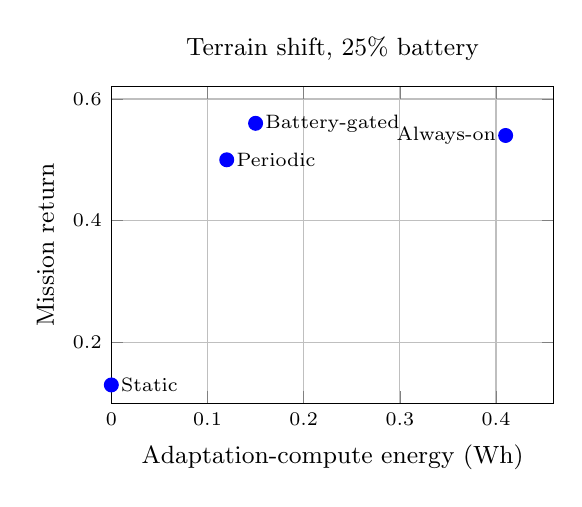
\begin{tikzpicture}
\begin{axis}[
  width=7.2cm,
  height=5.6cm,
  title={Terrain shift, 25\% battery},
  xlabel={Adaptation-compute energy (Wh)},
  ylabel={Mission return},
  xmin=0,
  xmax=0.46,
  ymin=0.10,
  ymax=0.62,
  grid=major,
  tick label style={font=\scriptsize},
  label style={font=\small},
  title style={font=\small},
]
\addplot[only marks, mark=*, mark size=2.5pt, color=blue] coordinates {(0.0,0.13) (0.12,0.5) (0.41,0.54) (0.15,0.56)};
\node[font=\scriptsize, anchor=west] at (axis cs:0.0,0.13) {Static};
\node[font=\scriptsize, anchor=west] at (axis cs:0.12,0.5) {Periodic};
\node[font=\scriptsize, anchor=east] at (axis cs:0.41,0.54) {Always-on};
\node[font=\scriptsize, anchor=west] at (axis cs:0.15,0.56) {Battery-gated};
\end{axis}
\end{tikzpicture}
&
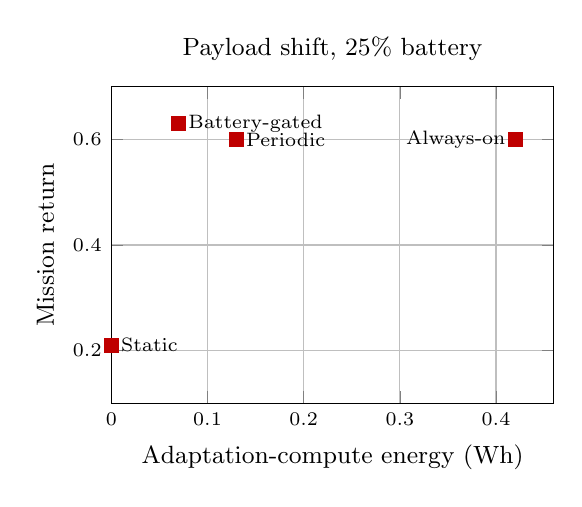
\begin{tikzpicture}
\begin{axis}[
  width=7.2cm,
  height=5.6cm,
  title={Payload shift, 25\% battery},
  xlabel={Adaptation-compute energy (Wh)},
  ylabel={Mission return},
  xmin=0,
  xmax=0.46,
  ymin=0.10,
  ymax=0.70,
  grid=major,
  tick label style={font=\scriptsize},
  label style={font=\small},
  title style={font=\small},
]
\addplot[only marks, mark=square*, mark size=2.5pt, color=red!75!black] coordinates {(0.0,0.21) (0.13,0.6) (0.42,0.6) (0.07,0.63)};
\node[font=\scriptsize, anchor=west] at (axis cs:0.0,0.21) {Static};
\node[font=\scriptsize, anchor=west] at (axis cs:0.13,0.6) {Periodic};
\node[font=\scriptsize, anchor=east] at (axis cs:0.42,0.6) {Always-on};
\node[font=\scriptsize, anchor=west] at (axis cs:0.07,0.63) {Battery-gated};
\end{axis}
\end{tikzpicture}
\end{tabular}
\end{document}
